\section{Foundations and Key Concepts}
\label{sec:background}

This work addresses the challenge of estimating the frequency of user visits within a spatial region of interest, $S$ (e.g., a city), while ensuring user privacy. The region $S$ is partitioned into a uniform grid $G$, where each cell $g_{i} \in G$ represents a distinct sub-region. For a set of users $U=\{u_{1}, u_{2}, ..., u_{n}\}$ moving within $S$ across discrete timestamps, the objective is to estimate the frequency $\hat{f}_{i}$ of visits to each cell $g_{i}$. Users generate true location reports $r_{i}$ at each timestamp, which are then anonymized locally using a Local Differential Privacy (LDP) mechanism $\Psi$ to produce private reports $\hat{r}_{i}=\Psi(r_{i})$ \cite{Filho2023FELIP}. An aggregator collects these private reports $\{\hat{r}_{i}\}_{i=1}^{|U|}$ and estimates the cell frequencies $\hat{f}_{i}$ using an estimator function $F(\cdot)$. Key concepts like LDP and Frequency Estimators, detailed below, form the basis of this approach. Table~\ref{tab:notations} summarizes commonly used notations. 

\begin{table}[tb]
  % \footnotesize
  \caption{Commonly Used Notations}
  \begin{tabular}{cp{5.9cm}}
    \toprule
    Notations&Meaning\\
    \midrule
    $S$ & Geo-space \\
    $g_i$,$G_i$ & Grid cell and Grid partition of $S$\\
    $u$,$U$ & User and the set of all users \\
    $t$,$T$ & Timestamp and set of all timestamps \\
    $f_i$,$\hat{f_i}$ & Frequency and frequency estimation for cell $g_i$\\
    $r_i$,$\hat{r}_i$ & User true report and user private report at each timestamp $i$ \looseness=-1\\
    $w$, $k$ & Window and grid size\\
  \bottomrule
\end{tabular}
\label{tab:notations}
\end{table}

\subsection{Local Differential Privacy}


Local Differential Privacy (LDP) differs significantly from the centralized model of Differential Privacy (DP) \cite{DBLP:conf/icalp/Dwork06} in where data perturbation occurs. In LDP, each user applies a randomized algorithm $\Psi$ locally to perturb their true data \textit{before} it is transmitted. Only the perturbed output is sent to the server, protecting the raw data and making LDP suitable for settings without a fully trusted data curator. This model is well-suited for longitudinal data, where users repeatedly report information over time, ensuring privacy at each step \cite{arcolezi2022improving}. \looseness=-1

\begin{definition}($\epsilon$ - LDP \cite{erlingsson2014rappor}) An algorithm
$\Psi(\cdot)$ satisfies $\epsilon$-local differential privacy, where $\epsilon \geq 0$, if and
only if for any pair of inputs $(v,v')$, and any set $R$ of possible outputs
of $\Psi$, we have
\begin{equation}
Pr[\Psi(v) \in R] \leq e^\epsilon Pr[\Psi(v') \in R]
\end{equation}
\label{def_ldp}
\end{definition} 

% \vspace{-0.6cm}

Intuitively, $\epsilon$\textit{-LDP} ensures that given the perturbed output in $R$,
it is not possible for the server or for an adversary to
distinguish whether the original true value was $v$ or $v'$ beyond
the probability ratio $e^\epsilon$. Here, $\epsilon$ controls the privacy level. Lower $\epsilon$ yields
stronger privacy. Analogous to central DP, LDP also benefits from key foundational properties, including robustness to post-processing and composition \cite{DBLP:journals/fttcs/DworkR14}.\looseness=-1

\begin{proposition}(Post-Processing)
    If $\Psi$ is $\epsilon$-LDP, then $f(\Psi)$ is also $\epsilon$-LDP for any function $f$.
\label{prop:post_processing}
\end{proposition}

\begin{proposition}(Sequential Composition)
     Let each $\Psi_i$ be an $\epsilon$-LDP mechanism, and $\Psi$ is the sequential composition $\Psi_1$,...,$\Psi_m$. Then, $\Psi$ satisfies $\sum_{i=1}^{m}  \epsilon$-LDP.
\label{prop:seq_processing}
\end{proposition}

\subsection{Frequency Estimator}
\label{sec:freq_estimator}

A frequency estimator is an LDP mechanism designed to estimate how often each value $r \in V$ appears in the dataset, where $V$ is the set of all possible values of a given attribute \cite{cormode2021frequency,bassily2015local}. A frequency estimator consists of two components: A sanitizer and an aggregator. The sanitizer is employed by users to locally perturb their data. An aggregator receives the perturbed data and estimates the frequencies regarding the input. Frequency estimators have been employed for a variety of different tasks such as answering range queries \citep{Filho2023FELIP}, identifying heavy hitters \citep{heavy_hitter_Zhu_24,qin2016heavy}, and the problem we attack in this paper, namely private queries on geospatial data \citep{geo_hong_21,laouir2024diapprox,tire2024answering}. \looseness=-1
\begin{figure}[htb]
    \centering
    \Description{Frequency estimation framework}
    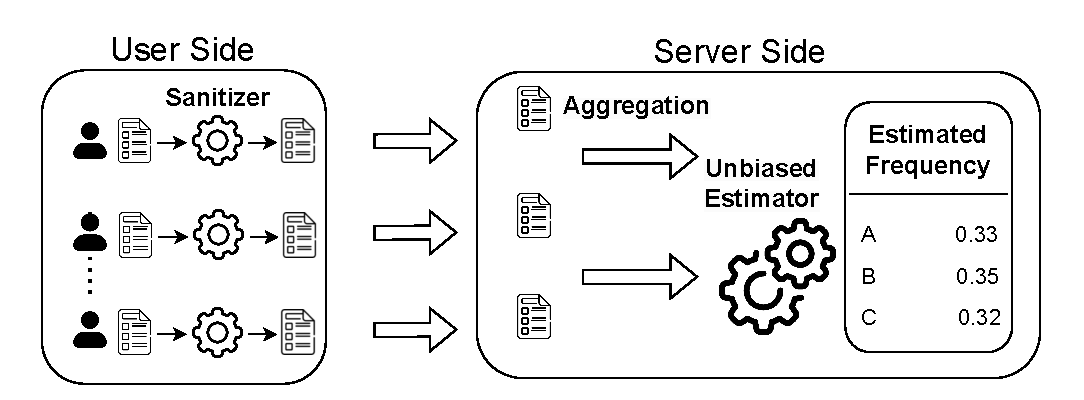
\includegraphics[width=0.9\linewidth]{sections/figures/freq_estimator.pdf}
    \caption{Frequency Estimator: users sending their sanitized report to the aggregator to estimate the frequency of values for a given attribute.}
    \label{fig:FE}
\end{figure}
% 
Figure \ref{fig:FE} illustrates a typical frequency estimator. In this example, the domain consists of three possible values: A, B, and C, which could represent items a user purchased, such as a doll, a car, or a dog. Each user applies a sanitization mechanism to their true report before submitting the sanitized version to the server. On the server side, the aggregator collects all sanitized reports and estimates the frequency of each value in the domain.

\subsection{Space Partitioning}
\label{sec:space_partition}

Spatial regions are commonly represented using map projections such as the Mercator projection, which converts latitude and longitude into a planar format \cite{peterson2014mapping}. While suitable for visualization, many analytical tasks require discretizing this continuous space into manageable units. Grid-based partitioning is a widely used approach due to its simplicity and effectiveness in dividing the region into uniform, contiguous cells \cite{shekhar2011identifying}.

Each cell represents a discrete sub-region of the original space, allowing any point (latitude and longitude) to be mapped to a specific cell. This structure supports efficient spatial queries, aggregations, and systematic data processing, particularly in high-density datasets \cite{yu2018geosparkviz}. \looseness=-1

To represent positions within the grid computationally, unary encoding can be applied. In a grid with \( k \) cells, each location is represented as a binary vector of length \( k \), with a 1 indicating the active cell and 0s elsewhere. For example, if a user is in cell 20 of a 100-cell grid, their position is encoded as a 100-bit vector with a 1 at index 20. Unary encoding is well-suited for privacy-preserving applications, as it enables straightforward integration with differential privacy mechanisms \cite{yang2023local}.

By discretizing spatial data and encoding positions in this manner, it becomes possible to anonymize and aggregate location information effectively, enabling privacy-aware frequency estimation and spatial analysis in sensitive domains.



